\documentclass{llncs}
\usepackage{amssymb}
\usepackage{graphicx}
%\usepackage[ruled,linesnumbered,boxed]{algorithm2e}
\usepackage{graphicx}
\usepackage{amsmath}
%\usepackage{mathtools}
%\usepackage{color}
\usepackage{tabularx}
\usepackage[colorlinks, linkcolor=blue, anchorcolor=blue, citecolor=green]{hyperref}
%\usepackage{booktabs}
\usepackage[table]{xcolor}
%\uespackage{colortbl}
\usepackage[vlined,ruled,linesnumbered]{algorithm2e}
\usepackage[tight,footnotesize]{subfigure}
\usepackage{fancyhdr}
\usepackage{lastpage}
\usepackage{layout}
\usepackage{multirow}
%\usepackage{ctex}
\usepackage{indentfirst}
%\footskip = 10pt
\pagestyle{fancy}
\chead{Group Project}
\lhead{CS214-Algorithm@SJTU}
\rhead{Instructor: Xiaofeng Gao}
\rfoot{}
\cfoot{Page \thepage \ of \pageref{LastPage}}
\addtolength{\headheight}{0.5\baselineskip}
\addtolength{\headwidth}{0\marginparsep}
\addtolength{\headwidth}{0\marginparwidth}
 \setlength{\parindent}{2em}


\title{Genetic Algorithm Combined with Local Search for Building Customized Bus-Booking Platform}
%\subtitle{The Sub-Title of Your Project \vspace{-3mm}}

\author{HaotianXue (518021910506, xavihart@sjtu.edu.cn) \\ 
SiyuanBian(518021910656, biansiyuan@sjtu.edu.cn) \\
YifanLiu (518021910609, sjtulyf123@sjtu.edu.cn)}
\institute{Department of Computer Science, \\ Shanghai Jiao Tong University, Shanghai, China}
 \setlength{\parindent}{2em}
\begin{document}
\bibliographystyle{splncs}

%\linespread{0.85}

%==============================================================================
\maketitle
\begin{abstract}\vspace{-5mm}
This project is aimed to solve some problems in customized bus-booking platform, including destination selection, route planning, order dispatch and pricing strategy. In this project we first choose departure station and destinations based on the real-world trace data, as well as filter part of the data to calculate the routes. After that, we convert our problem to Capacitated Vehicle Routing Problem (CVRP). Then we try to figure out the optimal solution of order dispatch and route planning by Google OR-Tools. Then, we utilize advanced genetic algorithm combined with local search to make route planning. We also introduce a pricing method for Customized Bus-Booking Platform. At last we simulate our algorithm on real-world data from DIDI GAIA Open Dataset and compare results of our algorithm with that calculated by Google OR-Tools solver.

\textbf{Keywords:} Genetic algorithm, Local Search, CVRP
\end{abstract}



\section{Problem Formalization}
\subsection{Formalization of V1, V2, and V3}
Given a complete graph $G = (V, E)$, we view each station as a vertex and view the road as edges. For all the edges $(v_i, v_j)$, there exists a cost called $D_{ij}$, which corresponds to the distance between the two stations. The bus fuel cost per kilometer is $c_b$. The cost per route of a bus is $c_r$. The bus fare price for one passenger from the departure station to station $v_j$ is $p_j$. 

There are $n$ customers in total, $m$ buses and the capacity of each bus is $L$.

A ``schedule'' is a function from a subset of Customers to the set of Bus. Suppose $A$ is a subset of customers, and $B$ is the set of all the buses, then $s$ is a schedule whose type is $A \rightarrow B$.

A ``valid'' schedule is the schedule in which each bus takes customers no more than its capacity. A ``full'' schedule is the schedule which is valid and all the customers can get on one bus. Obviously, a schedule $s$ is a full schedule iff $s$ is valid and the Domain of $s$ is the set of all customers.

Suppose the bus $b_j$ starts from $v_0$, stops at stations $\{v_1, v_2, \dots v_k\}$ and then drives back to $v_0$. The total distance of the bus is: 

\begin{equation}
totalDis_j = \sum_{i = 0}^{k-1}{D_{v_i, v_{i+1}}} + D_{v_k, v_0}
\end{equation}

The total profit of a schedule $s: A \rightarrow B$ can be expressed with the following formula:

\begin{equation}
Profit(s) = \sum_{i = 0}^{i<|A|}{p_j} - \sum_{i=0}^{i<|B|}{(c_b \times totalDis_i +c_r)}
\end{equation}

\begin{enumerate}
\item V1: Suppose $n \leq mL$, find a schedule which is \textbf{full} and has a largest profit.
\item V2: Find a schedule which is \textbf{valid} and has a largest profit.
\item V3: ``User dissatisfaction'' is determined by many factors. For example, if the customer's order is dropped, he has to wait for a long time for the next bus, which leads to dissatisfaction. Moreover, because the bus may detour to pass other stations, the passenger may spend more time on the bus than usual. So we calculate user dissatisfaction in the following way:
	\begin{equation}
	Diss = A e^{t_1/T_0} + B e^{(t_2 - t_n)/T_1}
	\end{equation}
In the equation, $t_1$ is the time a customer has wait for a bus, $t_2$ is the total time he spends on the bus, $t_n$ is the normal time he spends on the bus if no detour occurs. $A$ $B$, $T_0$, $T_1$ are all parameters which may be calculated based on real data.

Our goal is to maximize the following equation:
\begin{align*}
Goal(s) =& \alpha \times Profit - \beta \times Diss \\
	 =& \alpha (\sum_{i = 0}^{i<|A|}{p_j} - \sum_{i=0}^{i<|B|}{(c_b \times totalDis_i +c_r)}) - \beta(A e^{t_1/T_0} + B e^{(t_2 - t_n)/T_1})
\end{align*}
The parameters mean the same as above equations.
\end{enumerate}

\subsection{V4 Problem}
We may take into account the time of each bus ride. In this version, we add another constraint: a bus can start the second ride only when it has finished the previous ride, and has to take a break for $t_0$ (in the break, it may refuel and do some maintenance and so on). The bus always drives at the speed of $v$ on the road. Our goal is to schedule the buses so that we can make the largest profit in a certain interval of time. In the scheduling, we should not only consider which orders a bus should take, but should also decide the time each bus departs.

%In this version of ODRP problem, we may find that some orders are just too faraway that the bus can not get back to the station at a short time, so the ``Utilization rate'' of a bus may decrease.

\section{Decision Version}
Then we give the \textbf{Decision Version} of the problems. The contexts are the same as above.
\begin{enumerate}
\item V1: Suppose $n \leq mL$, find whether there exists a full schedule with a profit greater than $p$.
\item V2: Find whether there exists a valid schedule with a profit greater than $p$.
\item V3: Find whether there exists a valid schedule $s$ with $Goal(s) \geq g$.
\end{enumerate}

\section{Difficulty of the Problems}
The three versions of problems are all NP-complete. 

First, the problems are NP. Given a schedule, we know that the valid-schedule-check, the full-schedule-check, the profit calculation and user dissatisfaction calculation can all be done easily in polynomial time. So all the three versions of problems all have a polynomial-time certifier.

Then, We can prove the property of NP-complete by reducing from TSP(travelling salesman problem).
The TSP problem is stated as follows:

Given a Graph $G = (V, E)$, the weight of edge $(v_i, v_j)$ is $C_{ij}$. It is a minimization problem starting and finishing at $v_0$ after having visited each other vertex exactly once.

Also, we need to hypothesize that the triangle inequality always satisfies in the graph. That is to say, $C_{ij} \leq C_{ik} + C_{kj}$.

For the bus-schedule problem, we construct a complete graph $G' = (V, E')$. The new cost is defined below:
\begin{equation}
D(v_i, v_j) = 
		\begin{cases}
		C_{ij},\quad if\ (v_i, v_j) \in E\\
		\inf,\quad otherwise
		\end{cases}
\end{equation}
We suppose $m = 1$, $c_r = 0$, $L >> n$, the bus fee of each destination $p_j$ is also far larger than $c_b$.

\begin{enumerate}
\item For problem V1, we only have to prove the following lemma:
\begin{lemma}
There exists a most profitable bus schedule which never stops at one station twice.
\end{lemma}
\begin{proof}
Because the triangle inequality satisfies, if a bus stops at one station twice, it can just pass that station at the second time. After this, the total cost will not increase.
\end{proof}
Then we can safely say that the most profitable bus schedule must follow the path found by the TSP problem, and the path found by the TSP problem also corresponds to the most profitable bus schedule.

So $TSP \leq BusSchedule\ V1 $. Because the TSP problem is NP-complete, so $BusSchedule\ V1$ is also NP-complete. 

\item The proof of V2 is the same as the proof of V1. Because $L$ is far larger than $n$, and $p_j$ is also far larger than $c_b$, we can claim that carrying a passenger is always more profitable than drop it. So the most profitable schedule is just one schedule that carries all the passengers.

\item As we defined above, $Dis = A e^{t_1/T_0} + B e^{(t_2 - t_n)/T_1}$, we can assign $A$ and $B$ as numbers approximate to $0$. So the second term in $Goal(s)$ is always approximate to $0$, and has no obvious effect on the result. The rest of the proof is just the same as V2.
\end{enumerate}

\section{CVRP}
In this section, we introduce a problem called CVRP problem (Capacitated Vehicle Routing Problem), which is a classic problem with much previous research. Quite a lot of methods have been proposed and evaluated to solve CVRP problem. CVRP problem is quite similar to our ODRP problem, and we will prove latter of this section that our problem can be converted to a CVRP problem.

A CVRP problem can be roughly stated as the following:

Given a route graph and the distance between any of the two vertices. On each vertices, there are several ``orders''. There are $m$ vehicles in total and each vehicle has a capacity limit. We need to find the route of each vehicle such that 
\begin{itemize}
\item All vertices are visited once, and all orders are picked
\item The vehicle capacity limit is always satisfied
\item The total distance of all vehicles should be as small as possible
\end{itemize}

Sometimes, however, the orders are just impossible to be all picked. In this situation, we have to devise a penalty function which punishes dropping orders. And the goal switches to minimizing the total distance plus the sum of the penalties for all dropped locations.

Our ODRP problem is quite similar to a CVRP problem. The only difference is that in our problem, one station can be passed several times. But in CVRP problem, each station can be passed only once.

Then we find a simple way to convert our problem to CVRP problem: we just ``split'' the orders at one specific location. For example, if in our ODRP problem, there are 10 orders at vertex $v$, we can convert $v$ to 10 new vertices $\{v_{0}, v_{1}, \dots v_{9}\}$. The new vertices are all at the same location as $v$, but on each new vertex, there is just \textbf{one} order. The correctness of the conversion is easy to prove. 

After this conversion, we can just solve our problem with all the methods which are devised to solve CVRP. 

However, after the conversion, the number of vertices increase a lot, and the complexity of the problem is also greatly increased. So when the amount of data increases, the conversion is not always satisfactory. But after some analysis, we can find that we can find a similar conversion which can solve our problem with a good approximate:

We can find intuitively that in a good solution, a vertex cannot be visited by too may buses, because too many visits of a single vertex will cause much detour. So we can just split a vertex into several vertices, each of the new vertices have \textbf{more than one} orders. Then we use CVRP methods to solve the problem after conversion. We will show that the final result has a good precision.

In fact, the result may be better if we just do not split the vertex into vertices with only one order. Because by not splitting to scarcely, we somehow have introduced a prior assumption that in the optimal solution, a single vertex cannot be visited too many times. The prior assumption helps the convergence of our algorithm.

%\begin{equation}
%	x_i' = a[ \ln (x_i + b) + c]
%\end{equation}
% $a, b, c$ better satisfy the following equations:
%\begin{align*}
% &a[ \ln (x_{min} + b) + c] = 1\\
% &a[ \ln (x_{max} + b) + c] = capability\\
% &\frac{a}{\sqrt{x_{min}x_{max}} + b} \sim 1\\
%\end{align*}

\section{Station Selection}
\subsection{Destination Selection}
%We select the destinations according to number of orders in one region. 
We select the square region in which all the orders occur as the Region of Interest. Then, the Region of Interest is split into smaller squares with the side length of $5km$ (for Chengdu) and $10km$ (for Haikou). We calculate the number of orders in each of the small squares, and then sort the squares into a list according to the number of orders in them.

In the first attempt, we just choose the top 30 regions with the largest number of orders. However, we find that the selected regions are nearly all clustered in the city center. It is a bad choice because we will just lose the orders in the suburb, and the distance between destinations are too small.

In our optimized attempt, we choose top 10 regions with the largest number of orders. Then, we choose the rest 20 locations starting at the $11$-th square in the list with the interval of $1$. (That is to say, we choose $11$-th, $13$-th, $\dots$, $49$-th regions in the square list.) We use this means because in our data, we find that the neighboring squares in the square list are probably the ones also neighboring spatially. As a result, the interval can help us get more scarcely distributed destinations.

In this way, we have chosen the $30 $ destinations, and the $50$ destinations are chosen in the exactly same way. 

But the problem remains as how to allocate orders in the unselected squares? We tackle the problem by assigning the all the orders in one square to its closest destination. Because we need to calculate the distances between each pair of small squares, the assignment procedure is a little calculation-intensive. So we just use BFS (Breadth First Search) to get the well approximate result. The destination that is first reached in BFS can win all orders in the root square.

The approximation is correct because of the property of BFS search - it always finds the nearest locations first. The figure below will help understand it.
	\begin{figure}[htbp]
		\centering
		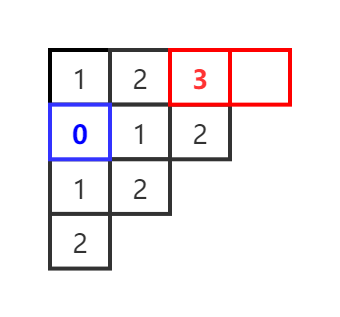
\includegraphics[width=1.5in]{destination_choice}
		\caption{The illustration of BFS in destination choosing}\label{fig:ill}
	\end{figure}

As shown in Figure \ref{fig:ill}, the red squares are destinations, and we want to assign the orders in the blue square to one of the red squares. Through BFS, we can find that the left red square can be reached with in three steps, so the left red square is the nearest picked destination of the blue square, which means we should assign all orders in the blue square to it.


\subsection{Departure Selection}
Just as the way we select destinations, we split the Region of Interest into smaller squares. Then we find the small square with the highest number of departure orders respectively as our departure station.
\begin{figure}
    \centering
    	\subfigure[30 destinations in Chengdu]{
			\begin{minipage}[t]{0.45\textwidth}
				\centering
				\includegraphics[width=\textwidth]{Chengdu30.PNG}
			\end{minipage}
		}
		\subfigure[50 destinations in Chengdu]{
			\begin{minipage}[t]{0.43\textwidth}
				\centering
				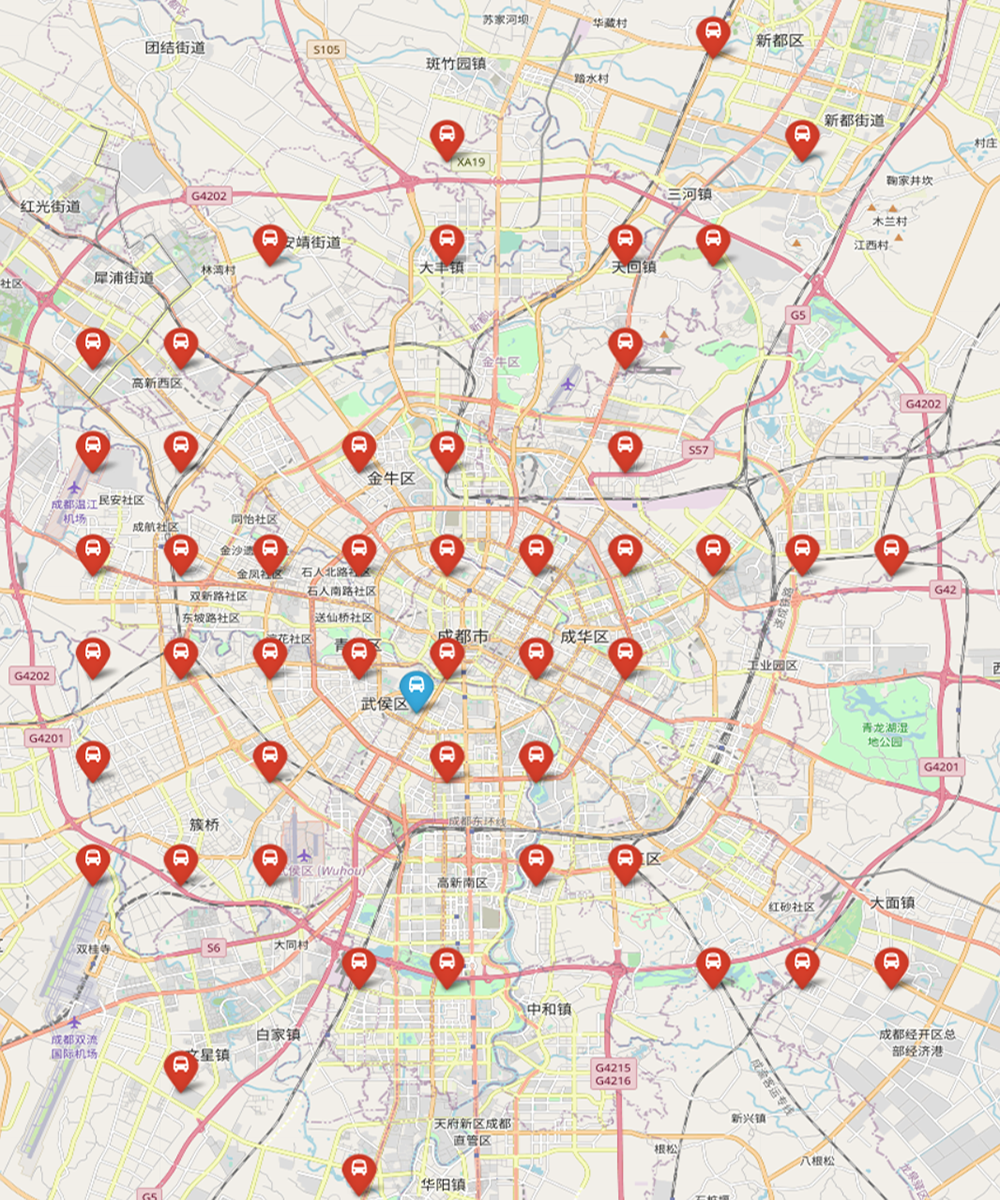
\includegraphics[width=\textwidth]{chengdu50.PNG}
			\end{minipage}
		}
		\subfigure[30 destinations in Haikou]{
			\begin{minipage}[t]{0.45\textwidth}
				\centering
				\includegraphics[width=\textwidth]{Haikou30.PNG}
			\end{minipage}
		}
		\subfigure[50 destinations in Haikou]{
			\begin{minipage}[t]{0.45\textwidth}
				\centering
				\includegraphics[width=\textwidth]{Haikou50.PNG}
			\end{minipage}
		}
    \caption{Destinations and departure station in Chengdu and Haikou}
    \label{fig:map}
\end{figure}

We map the departure station and destinations when we choose 30 and 50 destinations in Chengdu and Haikou to the real map, as is shown in Figure \ref{fig:map}. We could see the distribution of these stations vividly. The red points are destinations and the blue points are departure stations. The detailed data of departure station and destinations are in the data folder. 

\section{Order Records Filter}
Since $n>mL$, we need to pick a subset of orders based on the original orders we have. Considering the original distribution and number of orders, we use a kind of logistic function to process the original number of orders:
	\begin{align}
	n'_j=\lceil \frac{\frac{M}{L-1}e^{rn_j}}{\frac{e^{rn_j}}{L-1}+1}\rceil
	\end{align}
	
	where:
	\begin{itemize}
		\item $n'_j$ is the processed number of passengers whose destination $d_j$;
		\item $n_j$ is the original number of passengers whose destination $d_j$;
		\item $M$ represents the maximum number of processed data.
		\item $L$ and $r$ are parameters.
	\end{itemize}

	In Chengdu, we set $M=100,L=30,r=0.0003$; in Haikou, we set $M=100,L=30,r=0.00025$. The processed data and original data is shown in Table \ref{chengdu_logistic} and \ref{haikou_logistic}, the first line is the index of destinations.
	
	\begin{table}
		\caption{Orders in Chengdu}\label{chengdu_logistic}
		\centering
		\begin{tabular}{|c|c|c|c|c|c|c|c|c|c|c|c|c|c|c|c|}
			\hline
		index $j$&	1&2&3&4&5&6&7&8&9&10&11&12&13&14&15\\
		\hline
		$n_j$ &31769&18856&16676&15768&13697&13636&10246&7198&6706&4999&4996&4655&3698&3571&2627\\
		\hline
		$n_j$&100&91&84&80&68&68&43&24&21&14&14&13&10&10&8\\
			\hline
			index $j$&16&17&18&19&20&21&22&23&24&25&26&27&28&29&30\\
			\hline
			$n_j$&2150&2117&1637&1413&1620&1913&1875&1197&1277&777&1054&2241&872&663&3094\\
			\hline
			$n'_j$&7&7&6&6&6&6&6&5&5&5&5&7&5&5&9\\
			\hline
		\end{tabular}
	\end{table}

	\begin{table}
		\caption{Orders in Haikou}\label{haikou_logistic}
		\centering
		\begin{tabular}{|c|c|c|c|c|c|c|c|c|c|c|c|c|c|c|c|}
			\hline
			index $j$&	1&2&3&4&5&6&7&8&9&10&11&12&13&14&15\\
			\hline
			$n_j$&36772&28002&20459&19774&18722&17627&13893&13343&13190&12415&10032&7917&7676&4466&3069\\
			\hline
			$n'_j$&100&98&86&83&79&74&53&50&49&44&30&20&20&10&7\\
			\hline
			index $j$&16&17&18&19&20&21&22&23&24&25&26&27&28&29&30\\
			\hline
			$n_j$&2157&1892&1609&1488&1352&1029&896&999&970&611&573&398&600&591&319\\
			\hline
			$n'_j$&6&6&5&5&5&5&5&5&5&4&4&4&4&4&4\\
			\hline
		\end{tabular}
	\end{table}

\section{Optimal Solution Design and Results}
\subsection{Algorithm Design Using OR-Tools}
    We have converted our problem into the CVRP problem. So we just need to solve the converted CVRP problem. We use the Google OR-Tools ~\cite{ortools} in this project, which contains a VRP problem solver. The solver takes the positions of different locations, the orders to different locations, the capacity of each bus, and the total number of buses as input. Then it will output the detailed route, passengers and distance of each bus. It will also output the total distance and total passengers. 
	
	If we split the orders in every destination using the method we described above, we could use this solver to solve our problem. In order to get the optimal solution, we need to split the original orders into many pieces of one order. For example, if there are 4 orders in destination (1,1) originally, we split it into 4 ``destinations''. The position of each destination is also (1,1) and contains 1 order. The source code is shown in the appendices.
	
	The we use our optimal solver to estimate the computer's computing ability reach the physical limit to compute an optimal solution when $n,m,D$ increases. We know that when $n$ increases, we need more buses to satisfy all orders, so $m$ also increases. Besides, when $n$ increases, we need to split a destination to much more same pieces, and this change equals to the increase of $D$. Therefore, we choose to fix $D=30$, $L=30$ and increase $n$, to see when it reaches the computing ability to compute an optimal solution. We set the time limit to 10 minutes. If the solver runs for more than 10 minutes, we consider this $n$ is larger than the computing ceiling because we need much more time to list all solutions to find the best one. It turns out that when $n\approx3300$, the solver takes about 10 minutes to find the optimal solution. When $n>3400$, it would take more than 10 minutes to find the optimal solution. Therefore, the limit is around $3300\sim 3400$.
	
\subsection{Results of Our Optimal Solver}
    Since we choose 30 destinations, the destinations locations are the same as those of 30 destinations in the above section. We calculate the distance of matrix of all destinations and departure station. The detailed data could be found in the file \textit{distance matrix.txt}.

    We set $L=20,25,30$ respectively and use the orders processed above. We put the locations of destinations of 30 points and the selected departure station into our solver. We use Python to visualize our routes and they are shown in Figure \ref{opt_chengdu} and \ref{opt_haikou}, $L$ and $m$ represent the capacity of a bus and the number of the buses needed at least. The number on the node represents the index of destination, and the number beside the node represents the number of passengers to this destination. The detailed routes are in the file \textit{chengdu routes.txt, haikou routes.txt}.
	
	\begin{figure}[h]
		\centering
		\subfigure[$L=20,m=37$]{
		\begin{minipage}[t]{0.32\textwidth}
			\centering
			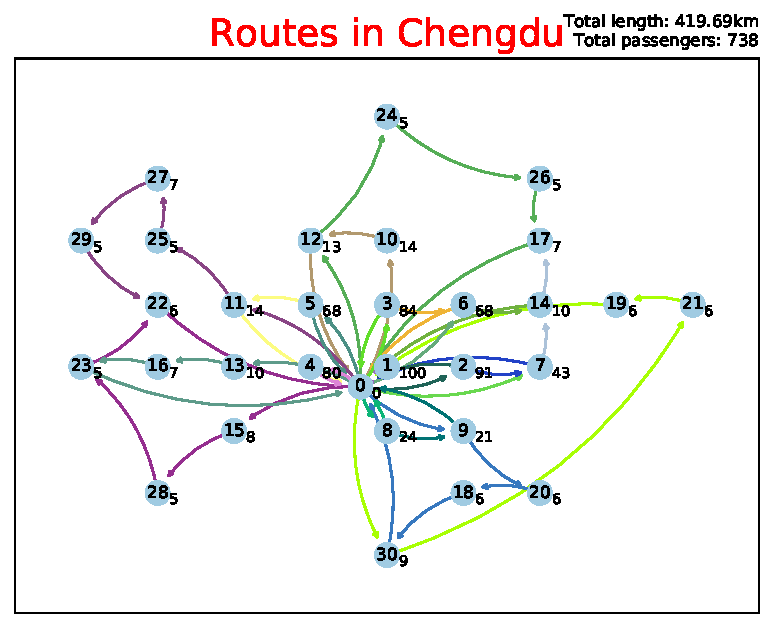
\includegraphics[width=\textwidth]{CVRP_chengdu_100_20.pdf}
		\end{minipage}
		}
		\subfigure[$L=25,m=30$]{	\begin{minipage}[t]{0.32\textwidth}
				\centering
				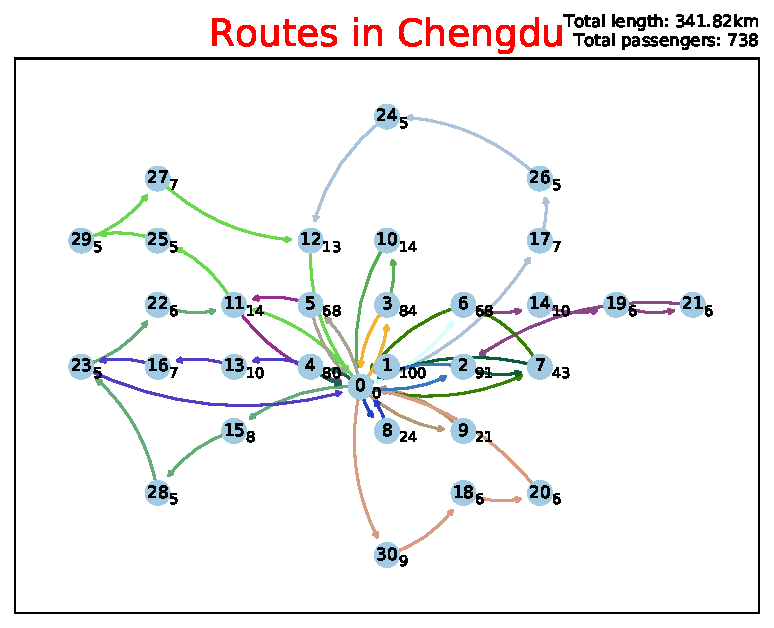
\includegraphics[width=\textwidth]{CVRP_chengdu_100_25.pdf}
		\end{minipage}}
		\subfigure[$L=30,m=25$]{	\begin{minipage}[t]{0.32\textwidth}
				\centering
				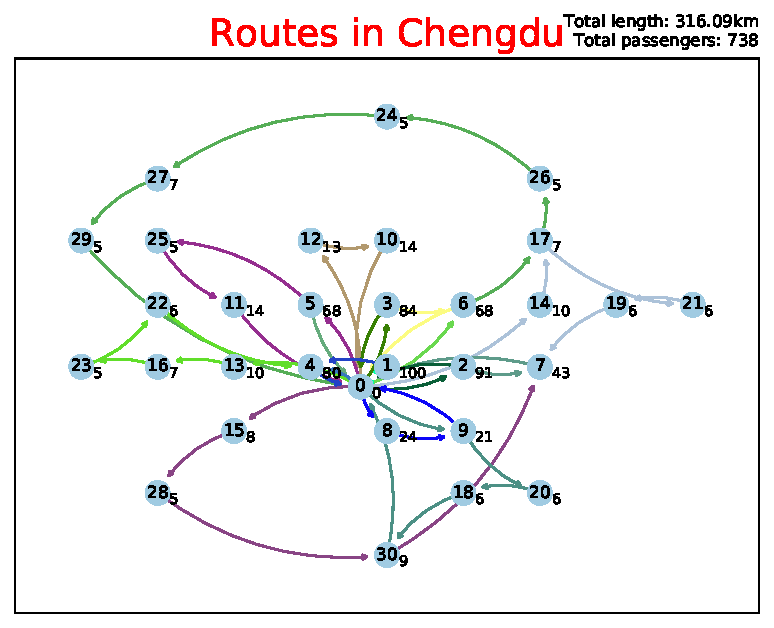
\includegraphics[width=\textwidth]{CVRP_chengdu_100_30.pdf}
		\end{minipage}}
		\caption{Visualization results in Chengdu}\label{opt_chengdu}
	\end{figure}

	\begin{figure}
		\centering
			\subfigure[$L=20,m=44$]{
			\begin{minipage}[t]{0.32\textwidth}
				\centering
				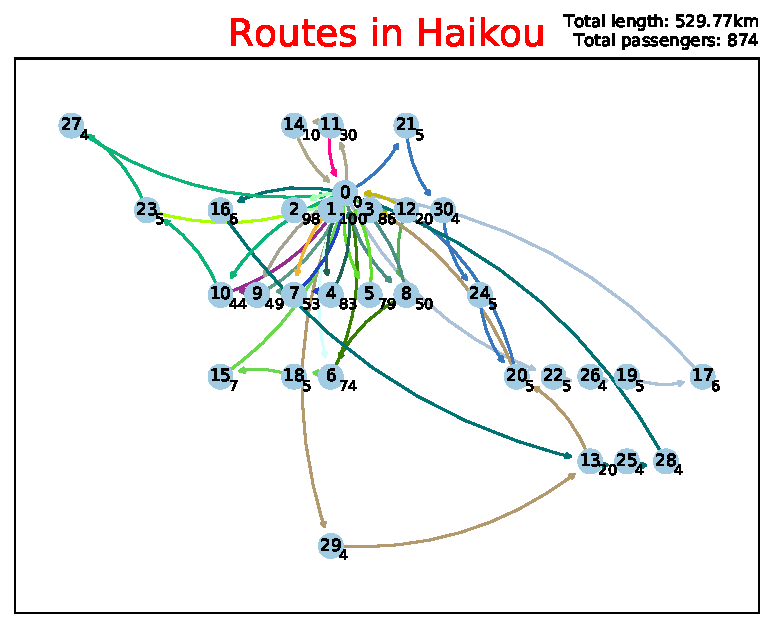
\includegraphics[width=\textwidth]{CVRP_haikou_100_20.pdf}
			\end{minipage}
		}
		\subfigure[$L=25,m=35$]{	\begin{minipage}[t]{0.32\textwidth}
				\centering
				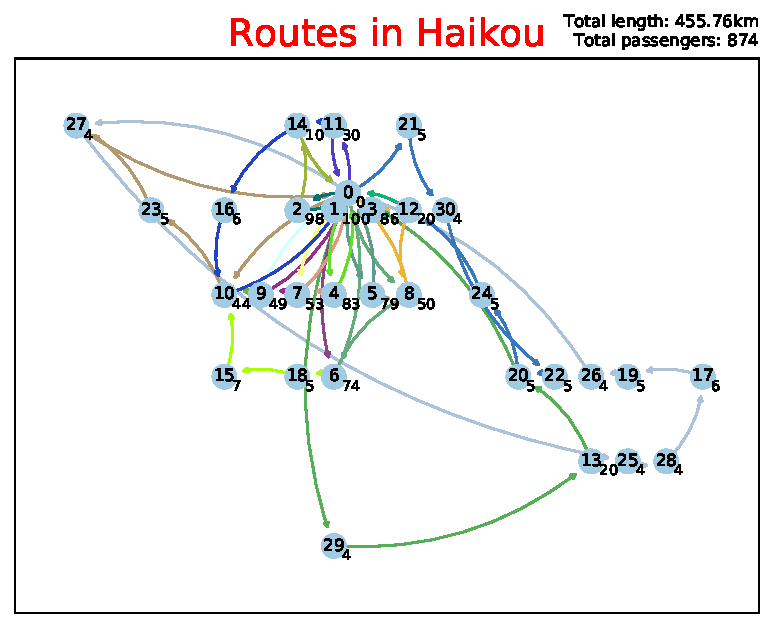
\includegraphics[width=\textwidth]{CVRP_haikou_100_25.pdf}
		\end{minipage}}
		\subfigure[$L=30,m=30$]{	\begin{minipage}[t]{0.32\textwidth}
				\centering
				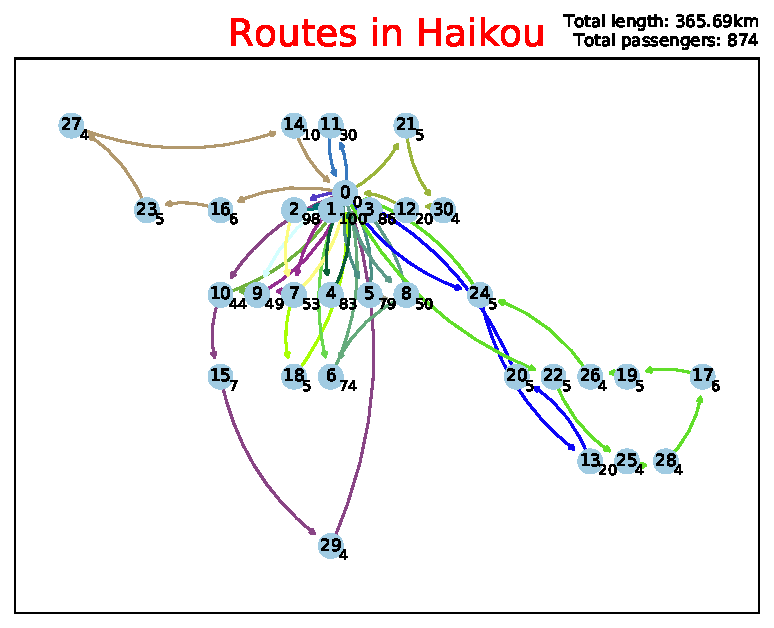
\includegraphics[width=\textwidth]{CVRP_haikou_100_30.pdf}
		\end{minipage}}
		\caption{Visualization results in Haikou}\label{opt_haikou}
	\end{figure}

    From the results of these real data, we could conclude that we had better use buses that have a larger $L$ to reduce the total route distance. Besides, we need to set $m$ as small as possible. 

\section{Genetic Algorithm}

\subsection{Basics}
We use Genetic Algorithm to solve ODRP-V2.

Genetic algorithm (GA) is a meta-heuristic algorithm inspired natural selection. In the algorithm, we represent each possible solution as an  individual with a chromosome. In each cycle, we do crossover (mixing genes from two ``parent'' individuals) and mutation (changing part of one individual's chromosome randomly). With well-designed algorithms, after some cycles, we can finally find a fine offspring out of a lot of comparable worse ancestors. The chromosome of that offspring is just the solution we are about to find.

In our problem, we represent each solution as a chromosome consisting of several routes, each containing the destinations that should be visited in the same order as they appear. Then we will introduce each part of our algorithm in detail.


\subsection{Fitness}
As the name suggests, the fitness of a solution indicates the quality of the solution. Intuitively, we may think that the solution with shorter total distance is the one with higher fitness value. But in reality, the fitness function fails in dealing with infeasible solutions. 

It should be noted that in our algorithm, we also allow temporary infeasible solutions which do not meet the requirement of total capacity of a bus. This is because the temporary infeasible solutions may help diversify the solution set, and help jump out of local optimal, to be more theoretical, this can expand our searching space, which may will make the convergence process faster. But the number temporary infeasible solutions cannot become too large, or it will squeeze out the feasible solutions.

Considering the infeasible solutions, we use a new fitness function both considering the distance of solution and punishing the infeasible solutions the same as in paper \cite{ga}, which take into considerations the iteration number. The fitness function is shown below:
\begin{equation}
f_s = \sum_{r\in s} cots_{s, r} + \alpha \cdot \frac{it}{IT}\sum_{r\in s}{(\max(0, totdem_{s,r} - cap))^2}
\end{equation}

where
\begin{itemize}
\item \textit{it}: is the current iteration, 
\item \textit{IT}: denotes the total number of iterations, 
\item \textit{$totdem_{r, s}$:} is the total demand of route $r$ in solution $s$, 
\item \textit{cap}: represents the uniform capacity of the vehicles, 
%\item \textit{best}: is the total cost of the best solution in the beginning 
%\item \textit{$dem_c$}: denotes the demand of customer $c \in s$
\end{itemize}
where $\alpha$ is a hyperparameter, and through experiment, we find that $\alpha = 0.1$ is a sound choice.
%%%%%%%%%%%%%%%%%%%% NEED CHANGING !!!!!!!!!!!!! %%%%%%%%%%%%%%%%%%%%%%%%%%%%%%
\subsection{Initialization}
The initial population is selected by greedy algorithm with some randomness. The algorithm will always choose the nearest destination available with probability of $0.9$, and choose randomly with probability of $0.1$. In this way, we ensure that the initial population is good enough to help produce the quick convergence, but is not ``too good'' so that those initial solutions may become predominant in the population at early stage, and make our algorithm stuck in local optimal.

\subsection{Crossover}
We only implement crossover in the solutions whose fitness ranks in the first quarter in population. That helps us seduce the amount of calculation as well as get comparably better descendants. 

Instead of using simple random crossover, we make some optimizations. We can learn intuitively that in a good solution, each bus may never  drive immediately to a destination too far away, but only drive to close destinations first. So in our crossover, we want our algorithm to favor those solutions with routes having nearer destinations. Inspired by the idea, we introduce a concept called ``Bounding box'' which represents the smallest rectangle an entire route fits in. Higher overlap rate between bounding boxes indicates higher closeness between two route. So when we talk about the overlap between two routes in the following part, we are actually talking about the overlap between two bounding boxes.

The specific crossover algorithm is shown here. First, we select two parent genes $P_1$ $P_2$ whose fitnesses rank in the first quarter in population. Then we randomly select a subroute from $P_2$, and find $3$ routes in $P_1$ having the biggest overlap with that subroute. Finally the subroute is inserted into one of the three routes which will produce a solution with the smallest total demand.

\begin{minipage}[t]{0.80\textwidth}
       \begin{algorithm}[H]
           \KwIn{Two individuals(Solution) in the population: $S_i$, $S_j$}
           \KwOut{child $C$}
           
           copy $S_i$ to $C$
           
           randomly choose a route $R$ with $|R|>1$ in $S_j$
           
           randomly choose a sub-route $r$ of $R$
           
           \For{all nodes $v$ in $r$}{
               delete $v$ from $C$
               
               connect two  neighbours of $v$
           }
           
           $BBX$ = bound box of $r$
           
           \For{all routes $r_c$ in C}{
               update the top-3 routes $r_1, r_2, r_3$ which have the biggest bounding box area with $BBX$
           }
           
           choose the route $r_c$ with the minimized demand in $r_i(i\in \{1,2,3\})$
           
          \For{all edge $e$ in $r_c$}{
               update the best edge to insert $r$ between  as $e_0$ 
           }
           
           insert $r$ between $e_0$ 
          
           \Return{$C$}
           \caption{Crossover($S_i$, $S_j$)}
        \end{algorithm}
        \end{minipage} 




\subsection{Mutation}
Through mutation, we make random changes to a specific descendant. We randomly choose a subroute from one route, and plug it into a randomly chosen route within the same solution. The frequency of mutation, the length of the subroute and so on are all hyper-parameters.

\begin{minipage}[t]{0.80\textwidth}
       \begin{algorithm}[H]
           \KwIn{One individual(Solution) in the population: $S$}
           \KwOut{$S$ after mutation}
             randomly choose a node $v\in r$ in $S=\{r_i\}$
             
             delete $v$ from $S$
             
             u = rand(0,1)
             
             
            \If{u < 0.3}{
               choose edge $e=(v_1,v_2)\in r$ in to insert $v$ between $v_1$ and $v_2$ with the lowest cost
            }
            \Else{
                choose edge $e=(v_1,v_2)\in r_0 \in S-\{r\}$ in to insert $v$ between $v_1$ and $v_2$ with the lowest cost
            }
           \Return{$S$}
           \caption{Mutation($S$)}
        \end{algorithm}
        \end{minipage} 
        
\subsection{Local Search Algorithm (LSA)}
Local search is used to optimize each individual in the population to make it reach a locally optimal state, which will make the genetic-guided process more controllable and supervised.  

In our implementations, for each route $R = \{start,r1,r2...,r_n,end\}$ in the individual, we traverse all the $<(r_i,r_{i+1}), (r_j, r_{j+1})>$ pairs, reordering them by replacing edges 
 $ (r_j, r_{j+1})$ and  $(r_i,r_{i+1})$ with edges  $(r_i,r_{j})$ and $(r_{j+1}, r_{i+1})$ if this replacement will decrease the total cost. We do this until no changes happened in the process, which means we reach a local optimization for all single route.

Actually in CrossOver and Mutation we have already used LSA to polish the genetic process when we choose best node to insert.

\begin{minipage}[t]{0.80\textwidth}
       \begin{algorithm}[H]
           \KwIn{One route in individual(Solution): $R=[v_1,v_2,...,v_n]$}
           \KwOut{$S$ after LSA}
             saving = $n$
             
             \While{saving > 0}{
                 saving = 0
                 
                 \For{i from $1$ to $n-1$}{
                 
                    \For{j from $1$ to $i$}{
                    
                        \If{i == j + 1}{
                            Continue
                        }
                        DistSaving = $dist(v_{j}, v_{j + 1}) + dist(v_i, v_{i + 1}) - dist(v_j, v_{i}) - dist(v_{i + 1}, v_{j + 1})$
                     
                     \If(DistSaving > saving){
                         saving = DistSaving
                         besti = i
                         bestj = j
                     }
                    }
                 }
                 
                 \If{saving > 0}{
                    rearrange the path to $[v_1, v_2, ..., v_j, v_i, v_{j+1}, v_{i+1},..., v_{n}]$
                 }
             } 
           \Return{$S$}
           \caption{LSA($R$)}
        \end{algorithm}
        \end{minipage} 


\subsection{Steps for Genetic Algorithm}
Fig \ref{ga-fig} illustrates the steps of the GA combined with local search. After we initialize the population, we use LSA on them and sorted them by fitness. Then we begin the loop for set iterations, where we first choose from the first $\frac{1}{4}$ of the population and make the first half crossover with the second for certain probability, and generate children which has certain chance to mutate. Then we replace the last $\frac{1}{8}$ with the children.
resorted then population and go on with the loop.


\begin{minipage}[t]{0.80\textwidth}
       \begin{algorithm}[H]
           \KwIn{departure station, destination stations and distance matrix}
           \KwOut{$solution$}
           initialize a population $P = [S_1, S_2, ..., S_n]$ with $n$
           
           individuals
           
           iter = 0
           
           k = 0
           
           \For{$i$ from $1$ to $n$}{
             \For{all $r\in S_i$ }{
              LSA($r$)
             }
           }
           
           \While{iter < iteration}{
               iter += 1
               
               \For{$i$ from $1$ to $\lceil \frac{n}{8} \rceil$}{
                   j = i + $\lceil \frac{n}{8} \rceil$
                   
                   r = rand(0, 1)
                   
                   \If{r < crossProp}{
                       c = CrossOver($S_i$, $S_j$)
                       
                       r = rand(0, 1)
                       
                       \If{r < mutateProp}{
                          c = Mutation(c)
                       }
                      
                   }
                   
              
                     \For{all $r\in c$ }{
                        LSA($r$)
                         }
                     
                   
                    $P[n - k] = c$
                       
                    $k$ += $1$
                   
               }
               update best solution $BestSolution$
               
               sort $P$ in increasing order of fitness
           }
           \Return{$BestSolution$}
           \caption{Process of GA}
        \end{algorithm}
        \end{minipage} 

 
 
 
	\begin{figure}[htbp]
		\centering
		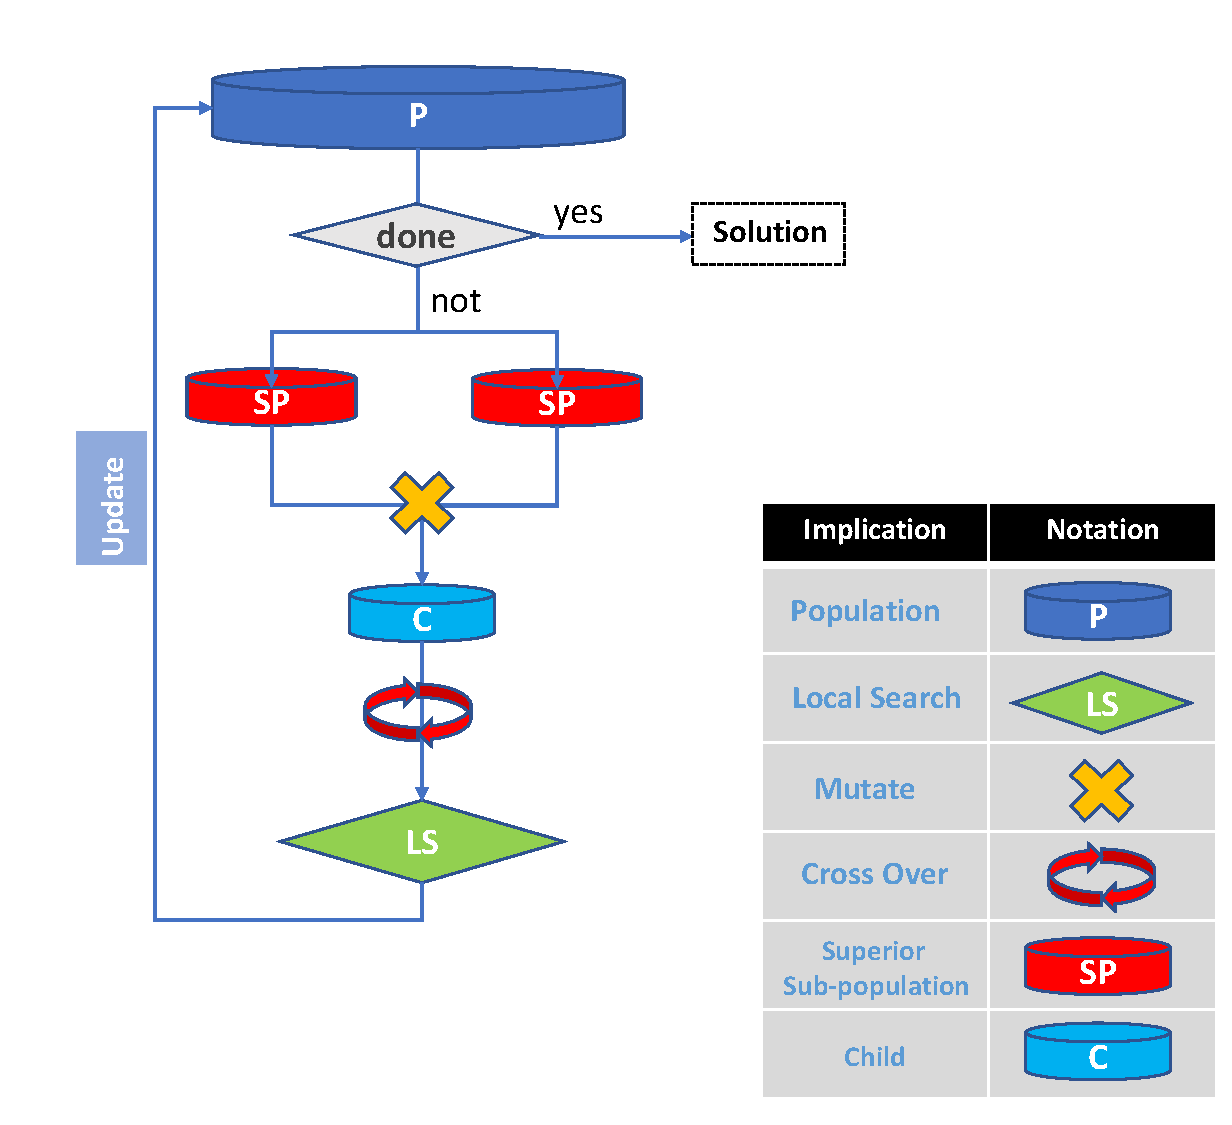
\includegraphics[width=4.5in]{ga.pdf}
		\caption{Steps for Genetic Algorithm}
		\label{ga-fig}
	\end{figure}
	
	\begin{figure}[htbp]
		\centering
		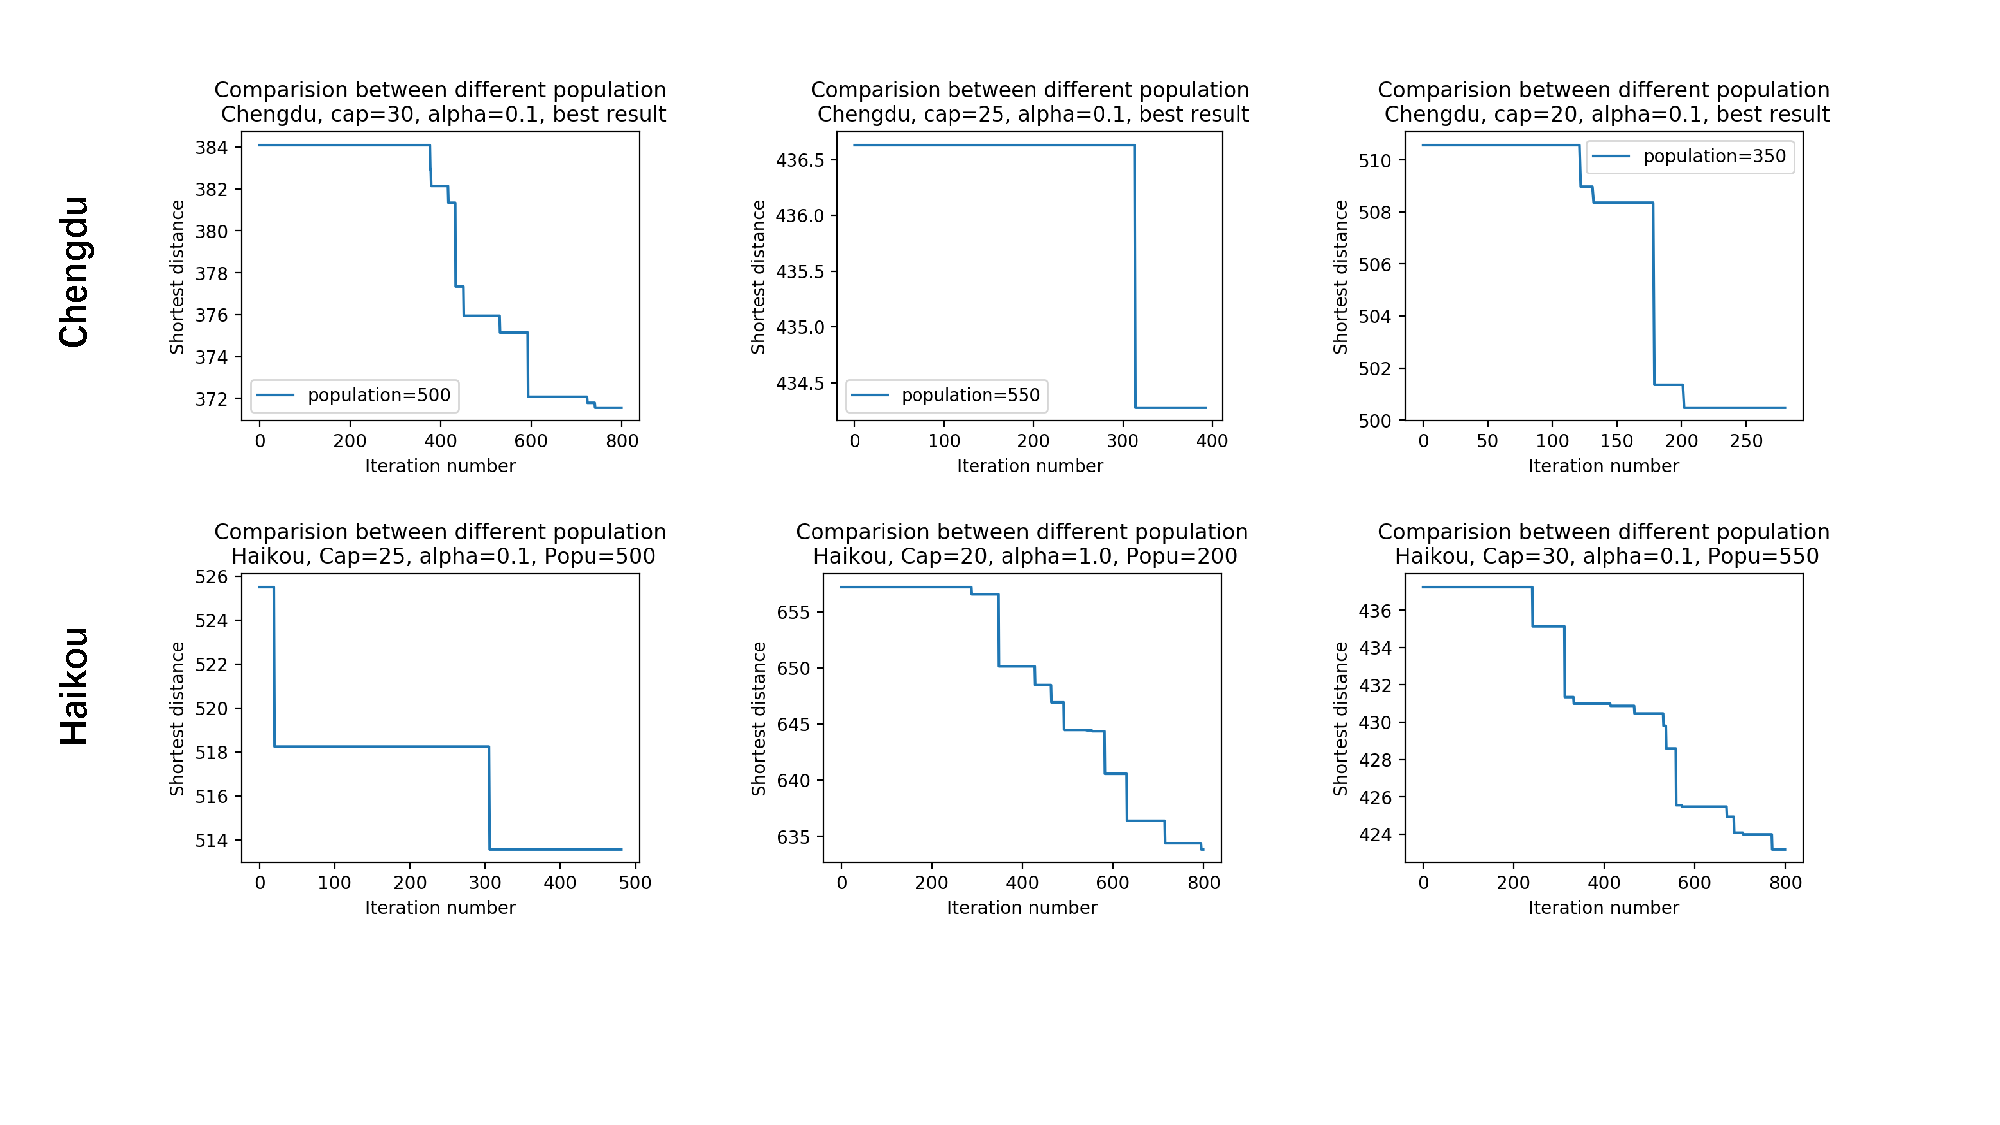
\includegraphics[width=5.5in]{GAplt.pdf}
		\caption{Iteration for genetic process}
		\label{plt-fig}
	\end{figure}
	
	\begin{figure}[htbp]
		\centering
		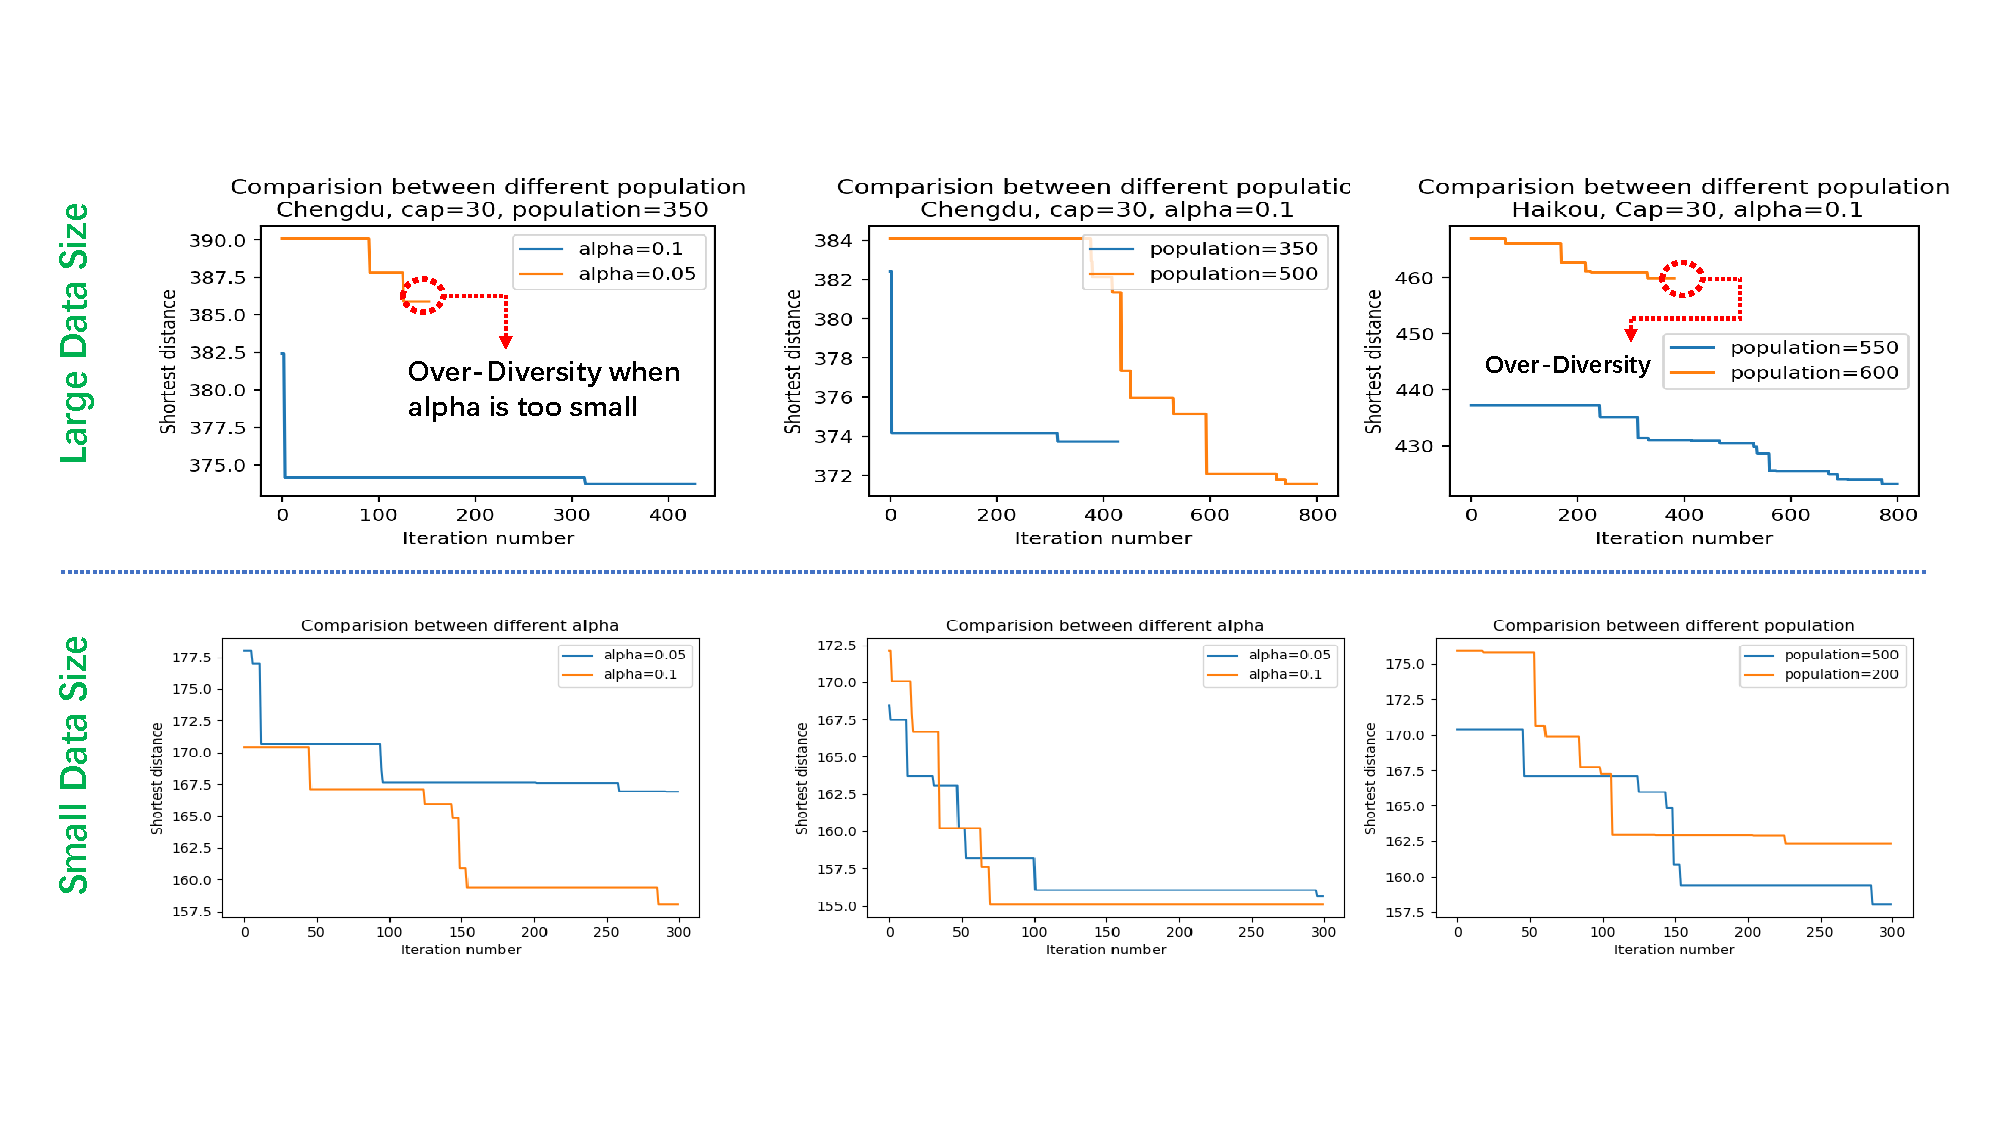
\includegraphics[width=5.5in]{cmp.pdf}
		\caption{Compare different parameters}
		\label{cmp-fig}
	\end{figure}



\begin{table}
\caption{Comparison of total distance between GA results and Or-Tools results}\label{tab1}
\centering
\begin{tabular}{|c|c|c|c|c|c|}
\hline
City &  Capability & Ortools &  \textbf{GA} & \textbf{Extra cost rate}\\
\hline
Chengdu & 20 & 419.69&500.47 &  19.2\% \\
Chengdu & 25 &341.82 &434.28 &  27.0\%\\
Chengdu & 30 &316.09 & 371.56 & 17.5\% \\
Haikou & 20 & 529.77&  634.38 & 19.7\% \\
Haikou & 25 & 455.76& 513.56 & 12.6 \\
Haikou & 30 &365.69 &385.89 & 5.52\% \\
\hline
\end{tabular}
\end{table}

\section{Pricing to Make Profit}
\subsection{Pricing Strategy}
	In order to maximize the total profit, beside from minimize the total distance of all routes, we need to design a reasonable pricing mechanism. We refer to the taxi price lists and bus fare rules. 
	
	The natural idea is that, like taxi pricing strategy, we set unit fare $w RMB/km$. For each passenger in each route, we compute the route distance from departure point to the passengers destination, and multiply the distance by $w$. However, this strategy has 2 problems. Firstly, the passengers to the same destination may be in different buses and different routes based on our algorithm, so they may have to pay different values, which is irrational. Secondly, since the route of the bus is a cycle, some destinations close to departure point could be visited later than the destinations that are far away from the departure point. This may cause the dissatisfaction of passengers.
	
	Therefore, we design a better algorithm based on the natural idea. We set unit fare $w RMB/km$ but ignore the difference of routes. We just calculate the direct distance of the destination of the passenger to the departure point, and multiply it by $w$. Then we could get the expression of total profit:
	\begin{align}\label{cost}
	\text{total profit}&=\text{total fares}-\text{total cost}\nonumber\\
	&=\sum_{j}p_j\times n_j-l\times c_b-m\times c_r\nonumber\\
	&=\sum_{j}w\times dis_{j}\times n_j-l\times c_b-m\times c_r
	\end{align}
	
	where:
	\begin{itemize}
		\item $p_j$ is the bus fare price for one passenger from the departure station to station $d_j$;
		\item $n_j$ is the number of passengers whose destination is $d_j$;
		\item $l$ is the total distance of all routes;
		\item $c_b$ is the bus fuel cost per kilometer;
		\item $m$ is the number of buses;
		\item $c_r$ is the cost per route of a bus;
		\item $w$ is the unit price per kilometer;
		\item $dis_j$ is the earth distance from destination $d_j$ to departure point.
	\end{itemize}
	
\subsection{Profit and Comparison With Taxi}
    	According to the taxi price in Chengdu~\cite{chengdu_taxi} and Haikou~\cite{haikou_taxi}, the oil price of the traditional bus~\cite{oilprice}, and other cost (like salary of bus drivers~\cite{salary}, maintenance of the bus, cost of buying a bus) per route~\cite{othercost}, we set $w=2,c_b=1.8,c_r=220$. In reference ~\cite{othercost}, the Life Cycle Cost (LCC) of a bus is 8 billion. It contains almost all the cost a bus could generate during 10 years. Then we could do calculation to figure out the other cost of a bus per route $c_r$.
	
	Then we could use Equation \ref{cost} to calculate total fares, total cost and total profit based on the optimal solver and GA results. We list these values in Table \ref{cost_table}. Since the fares are only affected by the distance, so the total fares are not affected by the capacity $L$ of the buses and the routes.
	\begin{table}
		\centering
		\caption{Total fares, cost and profit in Chengdu and Haikou}\label{cost_table}
		\begin{tabular}{|c|c|c|c|c|c|c|c|}
			\hline
			 &\multirow{2}{*}{L}&\multicolumn{3}{c|}{Optimal Solver} & \multicolumn{3}{c|}{GA}\\
			 \cline{3-8}
			 &&Total fares&Total cost&Total profit&Total fares&Total cost&Total profit\\
			 \hline
			 \multirow{3}{*}{Chengdu}&20&7386&8895&-1509&7386&9700&-2314\\
			 \cline{2-8}
			 &25&7386&7215&170&7386&8041&-655\\
			 \cline{2-8}
			 &30&7386&6068&1317&7386&6827&559\\
			 \hline
			 \multirow{3}{*}{Haikou}&20&9464&10633&-1169&9464&11699&-2235\\
			 \cline{2-8}
			 &25&9464&8520&943&9464&8843&621\\
			 \cline{2-8}
			 &30&9464&7258&2205&9464&8021&1443\\
			 \hline
		\end{tabular}
	\end{table}

	We could see from Table \ref{cost_table} that when the fares remain unchanged, and the capacity of buses increases, we tend to use fewer bus and shorter distance, so the total cost would decrease, and the total profit would increase. Therefore, using the bus that has a larger capacity would increase the profit dramatically.
	
	After that, we compare our pricing strategy with the pricing strategy of taxi. Here we list the pricing strategy of taxi in Chengdu and Haikou:
	\begin{align}
	Price_{Chengdu}(x)=\begin{cases}
	9\quad x\leq 2\\
	9+1.9(x-2)\quad 2<x\leq 10\\
	24.2+2.85(x-10) x>10
	\end{cases}
	\end{align}
	\begin{align}
	Price_{Haikou}(x)=\begin{cases}
	10\quad x\leq 3\\
	10+2(x-3)\quad x>3
	\end{cases}
	\end{align}
	
	We could easily figure out that since our pricing strategy does not have ``basic price'' and $w=2$, taking taxi is undoubtedly more expensive than taking our buses. If we have larger $L$ and more passengers, we could even decrease $w$ to 1.6, which is much more cheaper than taxi. Therefore, our pricing strategy is reasonable and could make profit.
	
\section{Acknowledgements}
We will extend our gratitude to Professor Gao Xiaofeng, our teacher of \textit{Algorithm and Complexity} class. In the class, we have learned a lot about fascinating algorithms and computational complexity theory. That helps us analyse our problem and design a suitable algorithm in the project. We have also learned to consult the documents, study something alien to us and make assessment all by ourselves. Those abilities will not only make us write better projects, but also help us in our future study and research career.

We are also grateful to our teaching assistants. They always give us selfless help whenever we have problems. Their quick and helpful responses eliminate our misconception and help us get better results.

Our classmates also help us a lot. It is always rewarding to discuss with each other. They often inspire us with some new ideas, and we are always working together to learn more and deeper.

%
% ---- Bibliography ----
%
% BibTeX users should specify bibliography style 'splncs04'.
% References will then be sorted and formatted in the correct style.
%
% \bibliographystyle{splncs04}
% \bibliography{mybibliography}
%
\begin{thebibliography}{8}
\bibitem{ortools}
Google OR-Tools, \url{https://developers.google.cn/optimization/}

\bibitem{chengdu_taxi}
Taxi Price in Chengdu, \url{https://baijiahao.baidu.com/s?id=1653543834837500081&wfr=spider&for=pc}

\bibitem{haikou_taxi}
Taxi Price in Haikou, \url{https://touch.go.qunar.com/utilinfo/407?destId=300148&destType=1}

\bibitem{oilprice}
Global Petrol Price, \url{https://zh.globalpetrolprices.com/China/diesel_prices/}

\bibitem{salary}
The Salary of Bus Drivers, \url{https://www.douban.com/note/683752483/}

\bibitem{othercost}
Bus Cost, \url{https://www.zhihu.com/question/29759637}

\bibitem{ga}
A. S. Bjarnadottir, Solving the Vehicle Routing Problem with Genetic Algorithms, 2004

\bibitem{didi}
DIDI GAIA Open Dataset, \url{https://outreach.didichuxing.com/research/opendata/en/}

\end{thebibliography}
\end{document}
